\documentclass[a4paper,12pt]{article}
\usepackage[ukrainian,english]{babel}
\usepackage{ucs}
\usepackage[utf8]{inputenc}
\usepackage[T2A]{fontenc}
\usepackage{amsmath}
\usepackage{amsfonts}
\usepackage{graphicx}
\usepackage{wrapfig}
\usepackage{multirow}
\usepackage{flafter}
\usepackage{lscape}
\usepackage{rotating}
\usepackage{booktabs}
\newcommand\tab[1][1cm]{\hspace*{#1}}
\usepackage[left=20mm, top=20mm, right=10mm, bottom=20mm, nohead, nofoot]{geometry}
\usepackage{blindtext}
\begin{document}
\begin{titlepage}
\begin{center}
\large НАЦІОНАЛЬНИЙ ТЕХНІЧНИЙ УНІВЕРСИТЕТ УКРАЇНИ «КИЇВСЬКИЙ ПОЛІТЕХНІЧНИЙ ІНСТИТУТ» ФІЗИКО-ТЕХНІЧНИЙ ІНСТИТУТ	
\newline\newline\newline\newline\newline\newline\newline\newline\newline
\LARGE{ЛАБОРАТОРНА РОБОТА З ФІЗИКИ № 2.1\\ ВИВЧЕННЯ ЗАКОНІВ ОБЕРТАЛЬНОГО РУХУ НА ПРИКЛАДІ МАЯТНИКА ОБЕРБЕКА}
\newline\newline\newline\newline\newline\newline\newline\newline\newline
\end{center}
\flushright 
Виконала:\\
студент групи  ФІ-12\\
Бекешева Анастасія \\
Прийняв:\\
Долгошей В.Б.

\end{titlepage}
\newpage
\section{Обробка результатів експерименту}
\begin{table}[htp]
\caption{Expiriment 1}
\centering
\begin{tabular}{|c|c|c|c|c|c|c|c|c|c|c|c|}
\hline
$h$ & $R$ & $r$   & $M$   & $t_1$ & $t_2$ & $t_3$ & $<t>$ & $a$   & $T$   & $\beta$ & $K$   \\ \hline
0.4 & 0   & 0.043 & 0.053 & 1.846 & 1.857 & 1.826 & 1.843 & 0.236 & 0.507 & 5.477   & 0.022 \\ \hline
0.4 & 0   & 0.043 & 0.095 & 1.438 & 1.569 & 1.558 & 1.522 & 0.346 & 0.898 & 8.035   & 0.039 \\ \hline
0.4 & 0   & 0.043 & 0.135 & 1.217 & 1.2   & 1.235 & 1.217 & 0.540 & 1.250 & 12.555  & 0.054 \\ \hline
0.4 & 0   & 0.043 & 0.177 & 1.11  & 1.07  & 1.093 & 1.091 & 0.672 & 1.616 & 15.630  & 0.069 \\ \hline
\end{tabular}
\end{table}
\begin{table}[htp]
\centering
\caption{Expiriment 2}
\begin{tabular}{|c|c|c|c|c|c|c|c|c|c|c|c|}
\hline
$h$ & $R$ & $r$   & $M$   & $t_1$ & $t_2$ & $t_3$ & $<t>$ & $a$   & $T$   & $\beta$ & $K$   \\ \hline
0.4 & 0.1 & 0.043 & 0.053 & 3.377 & 3.367 & 3.363 & 3.369 & 0.070 & 0.516 & 1.639   & 0.022 \\ \hline
0.4 & 0.1 & 0.043 & 0.095 & 2.469 & 2.446 & 2.422 & 2.446 & 0.134 & 0.918 & 3.110   & 0.039 \\ \hline
0.4 & 0.1 & 0.043 & 0.135 & 2.039 & 1.94  & 1.962 & 1.980 & 0.204 & 1.295 & 4.744   & 0.056 \\ \hline
0.4 & 0.1 & 0.043 & 0.177 & 1.666 & 1.712 & 1.653 & 1.677 & 0.284 & 1.684 & 6.615   & 0.072 \\ \hline
\end{tabular}
\end{table}
\begin{table}[htp]
\caption{Expiriment 3}
\centering
\begin{tabular}{|c|c|c|c|c|c|c|c|c|c|c|c|}
\hline
$h$ & $R$ & $r$   & $M$   & $t_1$ & $t_2$ & $t_3$ & $<t>$ & $a$   & $T$   & $\beta$ & $K$   \\ \hline
0.4 & 0.2 & 0.043 & 0.053 & 6.066 & 5.861 & 5.95  & 5.959 & 0.023 & 0.518 & 0.524   & 0.022 \\ \hline
0.4 & 0.2 & 0.043 & 0.095 & 4.07  & 4.079 & 3.968 & 4.039 & 0.049 & 0.926 & 1.140   & 0.040 \\ \hline
0.4 & 0.2 & 0.043 & 0.135 & 3.351 & 3.373 & 3.467 & 3.397 & 0.069 & 1.314 & 1.612   & 0.056 \\ \hline
0.4 & 0.2 & 0.043 & 0.177 & 2.956 & 3.051 & 3.01  & 3.006 & 0.089 & 1.719 & 2.059   & 0.074 \\ \hline
\end{tabular}
\end{table}
На основі експериментів 1-3 побудуємо графіки залежності $K(\beta)$ і за допомогою лінійної апроксимації визначимо моменти інерції та моменти тертя.\\
\begin{center}
	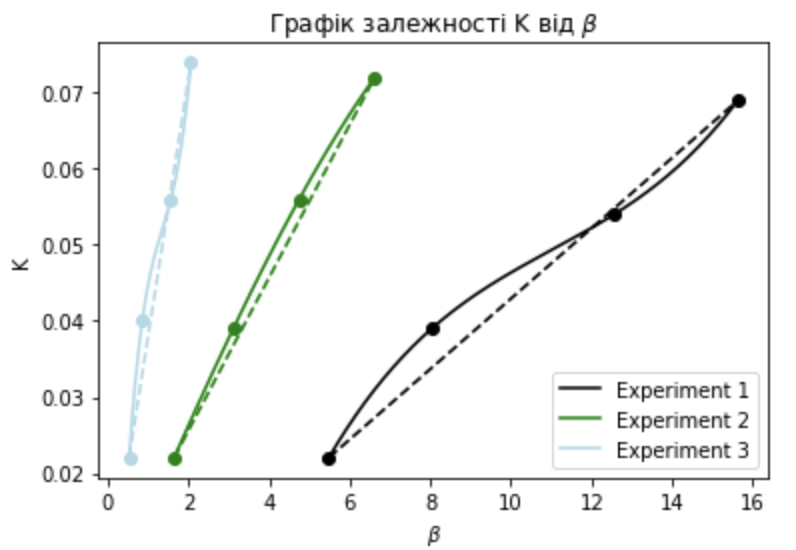
\includegraphics[width = 10cm]{graph5}
\end{center}
\newpage
За результатами апроксимації:
\begin{table}[htp]
\centering
\begin{tabular}{|c|c|}
\hline
$J$    & $K_{\textrm{тер}}$ \\ \hline
0.0337 & 0.0031             \\ \hline
0.01   & 0.0068             \\ \hline
0.0044 & 0.0001             \\ \hline
\end{tabular}
\end{table}\\
Тепер побудуємо графік залежності $J(R^2)$:
\begin{center}
	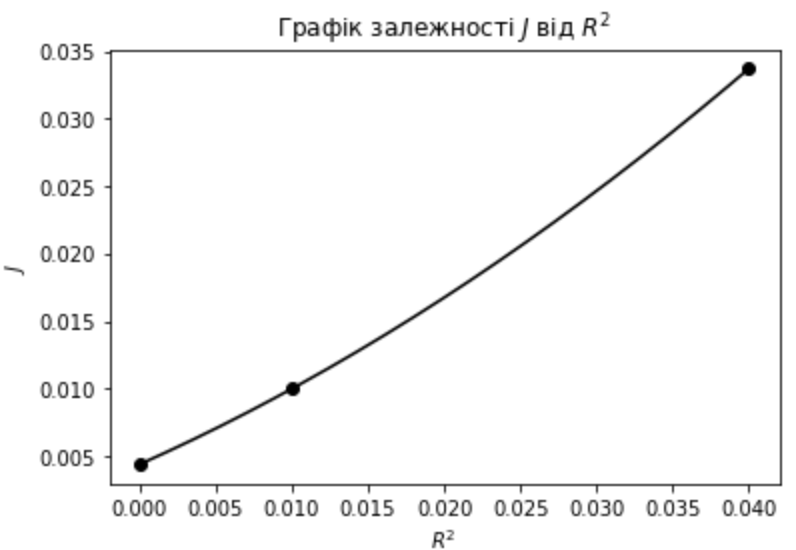
\includegraphics[width = 10cm]{graph6}
\end{center}
За результатами лінійної апроксимації, так як  $J=4mR^2+J_0+4J\beta$ та $J_0=0.004378165 \\
J\beta_{\textrm{екс}}= 2.7563\cdot10^{-5}$(кг$\cdot $м$^2$), \\
$J\beta_{\textrm{теор}}= 2.7\cdot10^{-5}$(кг$\cdot $м$^2$), \\
$E_{\textrm{абс}}= \pm(J\beta_{\textrm{теор}}-J\beta_{\textrm{екс}})$  (кг$\cdot $м$^2$) $=0.563\cdot10^{-5}$, \\
$E_{\textrm{відн}}=(J\beta_{\textrm{теор}}-J\beta_{\textrm{екс}})/J\beta_{\textrm{теор}}\cdot100\%=3.361$











\end{document}